% Options for packages loaded elsewhere
\PassOptionsToPackage{unicode}{hyperref}
\PassOptionsToPackage{hyphens}{url}
\PassOptionsToPackage{dvipsnames,svgnames,x11names}{xcolor}
%
\documentclass[
  10pt,
  ignorenonframetext,
]{beamer}
\usepackage{pgfpages}
\setbeamertemplate{caption}[numbered]
\setbeamertemplate{caption label separator}{: }
\setbeamercolor{caption name}{fg=normal text.fg}
\beamertemplatenavigationsymbolsempty
% Prevent slide breaks in the middle of a paragraph
\widowpenalties 1 10000
\raggedbottom
\setbeamertemplate{part page}{
  \centering
  \begin{beamercolorbox}[sep=16pt,center]{part title}
    \usebeamerfont{part title}\insertpart\par
  \end{beamercolorbox}
}
\setbeamertemplate{section page}{
  \centering
  \begin{beamercolorbox}[sep=12pt,center]{part title}
    \usebeamerfont{section title}\insertsection\par
  \end{beamercolorbox}
}
\setbeamertemplate{subsection page}{
  \centering
  \begin{beamercolorbox}[sep=8pt,center]{part title}
    \usebeamerfont{subsection title}\insertsubsection\par
  \end{beamercolorbox}
}
\AtBeginPart{
  \frame{\partpage}
}
\AtBeginSection{
  \ifbibliography
  \else
    \frame{\sectionpage}
  \fi
}
\AtBeginSubsection{
  \frame{\subsectionpage}
}
\usepackage{amsmath,amssymb}
\usepackage{iftex}
\ifPDFTeX
  \usepackage[T1]{fontenc}
  \usepackage[utf8]{inputenc}
  \usepackage{textcomp} % provide euro and other symbols
\else % if luatex or xetex
  \usepackage{unicode-math} % this also loads fontspec
  \defaultfontfeatures{Scale=MatchLowercase}
  \defaultfontfeatures[\rmfamily]{Ligatures=TeX,Scale=1}
\fi
\usepackage{lmodern}
\usetheme[]{Singapore}
\usefonttheme{serif}
\ifPDFTeX\else
  % xetex/luatex font selection
\fi
% Use upquote if available, for straight quotes in verbatim environments
\IfFileExists{upquote.sty}{\usepackage{upquote}}{}
\IfFileExists{microtype.sty}{% use microtype if available
  \usepackage[]{microtype}
  \UseMicrotypeSet[protrusion]{basicmath} % disable protrusion for tt fonts
}{}
\makeatletter
\@ifundefined{KOMAClassName}{% if non-KOMA class
  \IfFileExists{parskip.sty}{%
    \usepackage{parskip}
  }{% else
    \setlength{\parindent}{0pt}
    \setlength{\parskip}{6pt plus 2pt minus 1pt}}
}{% if KOMA class
  \KOMAoptions{parskip=half}}
\makeatother
\usepackage{xcolor}
\newif\ifbibliography
\usepackage{color}
\usepackage{fancyvrb}
\newcommand{\VerbBar}{|}
\newcommand{\VERB}{\Verb[commandchars=\\\{\}]}
\DefineVerbatimEnvironment{Highlighting}{Verbatim}{commandchars=\\\{\}}
% Add ',fontsize=\small' for more characters per line
\usepackage{framed}
\definecolor{shadecolor}{RGB}{248,248,248}
\newenvironment{Shaded}{\begin{snugshade}}{\end{snugshade}}
\newcommand{\AlertTok}[1]{\textcolor[rgb]{0.94,0.16,0.16}{#1}}
\newcommand{\AnnotationTok}[1]{\textcolor[rgb]{0.56,0.35,0.01}{\textbf{\textit{#1}}}}
\newcommand{\AttributeTok}[1]{\textcolor[rgb]{0.13,0.29,0.53}{#1}}
\newcommand{\BaseNTok}[1]{\textcolor[rgb]{0.00,0.00,0.81}{#1}}
\newcommand{\BuiltInTok}[1]{#1}
\newcommand{\CharTok}[1]{\textcolor[rgb]{0.31,0.60,0.02}{#1}}
\newcommand{\CommentTok}[1]{\textcolor[rgb]{0.56,0.35,0.01}{\textit{#1}}}
\newcommand{\CommentVarTok}[1]{\textcolor[rgb]{0.56,0.35,0.01}{\textbf{\textit{#1}}}}
\newcommand{\ConstantTok}[1]{\textcolor[rgb]{0.56,0.35,0.01}{#1}}
\newcommand{\ControlFlowTok}[1]{\textcolor[rgb]{0.13,0.29,0.53}{\textbf{#1}}}
\newcommand{\DataTypeTok}[1]{\textcolor[rgb]{0.13,0.29,0.53}{#1}}
\newcommand{\DecValTok}[1]{\textcolor[rgb]{0.00,0.00,0.81}{#1}}
\newcommand{\DocumentationTok}[1]{\textcolor[rgb]{0.56,0.35,0.01}{\textbf{\textit{#1}}}}
\newcommand{\ErrorTok}[1]{\textcolor[rgb]{0.64,0.00,0.00}{\textbf{#1}}}
\newcommand{\ExtensionTok}[1]{#1}
\newcommand{\FloatTok}[1]{\textcolor[rgb]{0.00,0.00,0.81}{#1}}
\newcommand{\FunctionTok}[1]{\textcolor[rgb]{0.13,0.29,0.53}{\textbf{#1}}}
\newcommand{\ImportTok}[1]{#1}
\newcommand{\InformationTok}[1]{\textcolor[rgb]{0.56,0.35,0.01}{\textbf{\textit{#1}}}}
\newcommand{\KeywordTok}[1]{\textcolor[rgb]{0.13,0.29,0.53}{\textbf{#1}}}
\newcommand{\NormalTok}[1]{#1}
\newcommand{\OperatorTok}[1]{\textcolor[rgb]{0.81,0.36,0.00}{\textbf{#1}}}
\newcommand{\OtherTok}[1]{\textcolor[rgb]{0.56,0.35,0.01}{#1}}
\newcommand{\PreprocessorTok}[1]{\textcolor[rgb]{0.56,0.35,0.01}{\textit{#1}}}
\newcommand{\RegionMarkerTok}[1]{#1}
\newcommand{\SpecialCharTok}[1]{\textcolor[rgb]{0.81,0.36,0.00}{\textbf{#1}}}
\newcommand{\SpecialStringTok}[1]{\textcolor[rgb]{0.31,0.60,0.02}{#1}}
\newcommand{\StringTok}[1]{\textcolor[rgb]{0.31,0.60,0.02}{#1}}
\newcommand{\VariableTok}[1]{\textcolor[rgb]{0.00,0.00,0.00}{#1}}
\newcommand{\VerbatimStringTok}[1]{\textcolor[rgb]{0.31,0.60,0.02}{#1}}
\newcommand{\WarningTok}[1]{\textcolor[rgb]{0.56,0.35,0.01}{\textbf{\textit{#1}}}}
\usepackage{graphicx}
\makeatletter
\def\maxwidth{\ifdim\Gin@nat@width>\linewidth\linewidth\else\Gin@nat@width\fi}
\def\maxheight{\ifdim\Gin@nat@height>\textheight\textheight\else\Gin@nat@height\fi}
\makeatother
% Scale images if necessary, so that they will not overflow the page
% margins by default, and it is still possible to overwrite the defaults
% using explicit options in \includegraphics[width, height, ...]{}
\setkeys{Gin}{width=\maxwidth,height=\maxheight,keepaspectratio}
% Set default figure placement to htbp
\makeatletter
\def\fps@figure{htbp}
\makeatother
\setlength{\emergencystretch}{3em} % prevent overfull lines
\providecommand{\tightlist}{%
  \setlength{\itemsep}{0pt}\setlength{\parskip}{0pt}}
\setcounter{secnumdepth}{-\maxdimen} % remove section numbering
\usepackage{multirow}
\ifLuaTeX
  \usepackage{selnolig}  % disable illegal ligatures
\fi
\IfFileExists{bookmark.sty}{\usepackage{bookmark}}{\usepackage{hyperref}}
\IfFileExists{xurl.sty}{\usepackage{xurl}}{} % add URL line breaks if available
\urlstyle{same}
\hypersetup{
  pdftitle={Module 1: Introduction},
  pdfauthor={Sara Martino, Department of Mathematical Sciences, NTNU},
  colorlinks=true,
  linkcolor={Maroon},
  filecolor={Maroon},
  citecolor={Blue},
  urlcolor={blue},
  pdfcreator={LaTeX via pandoc}}

\title{Module 1: Introduction}
\subtitle{TMA4268 Statistical Learning V2023}
\author{Sara Martino, Department of Mathematical Sciences, NTNU}
\date{11th January, 2024}

\begin{document}
\frame{\titlepage}

\begin{frame}{Acknowledgements}
\protect\hypertarget{acknowledgements}{}
\begin{itemize}
\tightlist
\item
  This course had been built up by Mette Langaas at NTNU in 2018 and
  2019 and revised by Stefani Muff in 2020-2023. I am using a some of
  their material, and material from her TAs, throughout the course.\\
  \vspace{2mm} \textbf{I would like to thank Mette and Steffi for the
  great work and for the permission to use her material!}
\end{itemize}

\(~\)

\begin{itemize}
\tightlist
\item
  Thanks to Julia Debik for contributing to this module page.
\end{itemize}
\end{frame}

\begin{frame}{Learning outcomes of TMA4268}
\protect\hypertarget{learning-outcomes-of-tma4268}{}
\begin{enumerate}
\item
  \textbf{Knowledge.} The student has knowledge about the most popular
  statistical learning models and methods that are used for
  \emph{prediction} and \emph{inference} in science and technology.
  Emphasis is on regression- and classification-type statistical models.
\item
  \textbf{Skills.} The student can, based on an existing data set,
  choose a suitable statistical model, apply sound statistical methods,
  and perform the analyses using statistical software. The student can
  present, interpret and communicate the results from the statistical
  analyses, and knows which conclusions can be drawn from the analyses,
  and what the caveats are.
\end{enumerate}
\end{frame}

\begin{frame}{Learning material}
\protect\hypertarget{learning-material}{}
\begin{enumerate}
[1)]
\item
  \textbf{The main learning source} is the textbook by James, Witten,
  Hastie, Tibshirani (2021, 2nd edition): ``An Introduction to
  Statistical Learning''. The textbook can be downloaded here:
  \url{https://www.statlearning.com/}

  \begin{itemize}
  \tightlist
  \item
    There are 15 hours of youtube videos by two of the authors of the
    book, Trevor Hastie an Rob Tibshirani. Links will be added to the
    module subpages.
  \end{itemize}
\item
  All the lecture notes (iPad notes will be made available online).
\item
  The R course here:
  \url{https://digit.ntnu.no/courses/course-v1:NTNU+IE-IMF+2023_AUG/about}
\item
  \textbf{Additional reading material will be clearly indicated in the
  modules and on the course page.}
\end{enumerate}
\end{frame}

\begin{frame}{Course page}
\protect\hypertarget{course-page}{}
All the relevant information for the course can be found here:

\url{https://wiki.math.ntnu.no/tma4268/2024v/start}

On each module page, all the relevant learning material and exercises
(incl.~solutions) will be provided in due time.
\end{frame}

\begin{frame}{The Statistical Learning Team 2024}
\protect\hypertarget{the-statistical-learning-team-2024}{}
\begin{block}{The TAs:}
\protect\hypertarget{the-tas}{}
\vspace{2mm}

\begin{itemize}
\tightlist
\item
  \href{https://www.ntnu.no/ansatte/kenneth.aase}{Kenneth Aaase}; PhD
  student
\item
  \href{https://www.ntnu.no/ansatte/daesoo.lee}{Daesoo Lee}; PhD student
\end{itemize}

\(~\)
\end{block}

\begin{block}{The Lecturers}
\protect\hypertarget{the-lecturers}{}
\vspace{2mm}

\begin{itemize}
\tightlist
\item
  \href{https://www.ntnu.no/ansatte/sara.martino}{Sara Martino};
  Associate Professor
\item
  \href{https://www.ntnu.edu/employees/stefanie.muff}{Stefanie Muff};
  Associate Professor
\end{itemize}
\end{block}
\end{frame}

\begin{frame}{Who is this course for?}
\protect\hypertarget{who-is-this-course-for}{}
\begin{block}{Primary requirements}
\protect\hypertarget{primary-requirements}{}
\(~\)

\begin{itemize}
\tightlist
\item
  Bachelor level: 3rd year students from Science or Technology programs,
  and master/PhD level students with interest in performing statistical
  analyses.
\end{itemize}

\vspace{2mm}

\begin{itemize}
\tightlist
\item
  Statistics background: TMA4240/45 Statistics, ST1101+ST1201
  (probability theory and statistical methods), or equivalent.
\end{itemize}

\vspace{2mm}

\begin{itemize}
\tightlist
\item
  No background in statistical software needed: but we will use the R
  statistical software extensively in the course. Knowing Python will
  make this easier for you!
\end{itemize}

\vspace{2mm}

\begin{itemize}
\tightlist
\item
  Advantage with knowledge of computing - for example an introductory
  course in informatics, like TDT4105 or TDT4110.
\end{itemize}
\end{block}
\end{frame}

\begin{frame}
\begin{block}{Overlap}
\protect\hypertarget{overlap}{}
\vspace{2mm}

\begin{itemize}
\tightlist
\item
  \href{https://www.ntnu.no/studier/emner/TDT4173\#tab=omEmnet}{TDT4173}
  Machine learning and case based reasoning: courses differ in
  philosophy (computer science vs.~statistics).
\end{itemize}

\vspace{2mm}

\begin{itemize}
\tightlist
\item
  \href{https://www.ntnu.no/studier/emner/TMA4267\#tab=omEmnet}{TMA4267}
  Linear Statistical Models: useful to know about multivariate random
  vectors, covariance matrices and the multivariate normal distribution.
  Overlap only for multiple linear regression (M3).
\end{itemize}
\end{block}
\end{frame}

\begin{frame}{About the course}
\protect\hypertarget{about-the-course}{}
\begin{block}{Focus: Statistical theory \textbf{and} doing analyses}
\protect\hypertarget{focus-statistical-theory-and-doing-analyses}{}
\(~\)

\begin{itemize}
\tightlist
\item
  The course has focus on \textbf{statistical theory}, but we apply all
  models and theory using (mostly) available function in R and real data
  sets.
\end{itemize}

\vspace{2mm}

\begin{itemize}
\tightlist
\item
  It is important that the student in the end of the course \textbf{can
  analyse all types of data} (covered in the course) - not just
  understand the theory.
\end{itemize}

\vspace{2mm}

\begin{itemize}
\tightlist
\item
  And vice versa - the student must also \textbf{understand} the model,
  methods and algorithms used.
\end{itemize}
\end{block}
\end{frame}

\begin{frame}
\begin{block}{Teaching philosophy}
\protect\hypertarget{teaching-philosophy}{}
~

\begin{itemize}
\tightlist
\item
  Divide the topics of the course into modular units with specific
  focus.
\end{itemize}

~

\begin{itemize}
\tightlist
\item
  This (hopefully) facilitates learning?
\end{itemize}

~

\begin{itemize}
\tightlist
\item
  Two weeks without lectures, time to work on the compulsory exercises.
\end{itemize}
\end{block}
\end{frame}

\begin{frame}
\begin{block}{Course content: The 12 Modules}
\protect\hypertarget{course-content-the-12-modules}{}
\vspace{4mm}

\begin{itemize}
\tightlist
\item
  \textbf{Module 1}: Introduction \& R course (this module)
\end{itemize}

\vspace{2mm}

\begin{itemize}
\tightlist
\item
  \textbf{Modules 2 - 11}:

  \begin{enumerate}
  [1)]
  \setcounter{enumi}{1}
  \tightlist
  \item
    Statistical learning
  \item
    Multiple linear regression
  \item
    Classification
  \item
    Resampling methods
  \item
    Model selection/regularization
  \item
    Non-linearity
  \item
    Tree-based methods 1
  \item
    Tree-based methods 2
  \item
    Unsupervised methods
  \item
    Neural networks (new in the course book edition 2)
  \end{enumerate}
\end{itemize}

\vspace{2mm}

\begin{itemize}
\tightlist
\item
  \textbf{Module 12}: Summing up
\end{itemize}
\end{block}
\end{frame}

\begin{frame}
\begin{block}{Learning methods, activities and grading}
\protect\hypertarget{learning-methods-activities-and-grading}{}
\(~\)

\begin{itemize}
\tightlist
\item
  Lectures, exercises and works (projects).
\end{itemize}

\(~\)

\begin{itemize}
\tightlist
\item
  The assessment is a 100\% final school exam.
\end{itemize}

\(~\)

\begin{itemize}
\tightlist
\item
  To be allowed to the exam, you need to reach \textbf{at least 60\% in
  both compulsory exercises}.
\end{itemize}

\(~\)

\begin{itemize}
\tightlist
\item
  Retake of examination may be given as an oral examination. The
  lectures are given in English.
\end{itemize}
\end{block}
\end{frame}

\begin{frame}
\begin{block}{The lectures}
\protect\hypertarget{the-lectures}{}
\vspace{4mm}

\textbf{Thursdays at 8.15-10.00 in EL6 and Fridays at 12.15-14.00 in
EL6}

\vspace{4mm}

\begin{itemize}
\tightlist
\item
  We have \(2\times 2\) hours of lectures every week (except when
  working with the compulsory exercises).
\end{itemize}

\vspace{2mm}

\begin{itemize}
\tightlist
\item
  See here
  \url{https://github.com/stefaniemuff/statlearning2/blob/main/TMA4268_schedule2024.pdf}
  for a tentative schedule.
\end{itemize}

\vspace{2mm}

\begin{itemize}
\tightlist
\item
  \textbf{I suggest that you always have your laptop handy for the
  lecture.} So you can run code or do an exercise in class.
\end{itemize}
\end{block}
\end{frame}

\begin{frame}
\begin{block}{The first week: The R course}
\protect\hypertarget{the-first-week-the-r-course}{}
\(~\)

\begin{itemize}
\tightlist
\item
  In this \textbf{first week of the course} you will have to work
  through parts 1-6 of the R course on the openEdX page here:
  \url{https://digit.ntnu.no/courses/course-v1:NTNU+IMF001+2020/course/}
\end{itemize}

\(~\)

\begin{itemize}
\tightlist
\item
  Log in with your Feide account (scroll a bit down).
\end{itemize}

\(~\)

\begin{itemize}
\tightlist
\item
  There is a discussion forum that you can use for the R course.
\end{itemize}
\end{block}
\end{frame}

\begin{frame}
\begin{block}{Recommended exercises}
\protect\hypertarget{recommended-exercises}{}
\vspace{4mm}

\textbf{Thursdays at 16.15-19.00 in EL6}

\vspace{4mm}

\begin{itemize}
\tightlist
\item
  For each module \emph{recommended exercises} are uploaded. These are
  partly

  \begin{itemize}
  \tightlist
  \item
    theoretical exercises (from book or not)
  \item
    computational tasks
  \item
    data analysis
  \end{itemize}
\end{itemize}

\vspace{2mm}

\begin{itemize}
\tightlist
\item
  These are supervised in the weekly exercise slots.
\end{itemize}

\vspace{2mm}

\begin{itemize}
\tightlist
\item
  Solutions will be provided to check yourself (no grading).
\end{itemize}

\vspace{2mm}

\begin{itemize}
\tightlist
\item
  Starting next week.
\end{itemize}

\(~\)
\end{block}
\end{frame}

\begin{frame}
\begin{block}{The compulsory exercises}
\protect\hypertarget{the-compulsory-exercises}{}
\vspace{4mm}

\begin{itemize}
\tightlist
\item
  We will have \textbf{two compulsory exercises/projects}.
\end{itemize}

\vspace{2mm}

\begin{itemize}
\tightlist
\item
  Both projects need to be completed, where at least \textbf{60\% of the
  points must be reached in both of them} to be admitted to the exam.
\end{itemize}

\vspace{2mm}

\begin{itemize}
\tightlist
\item
  The exercises/projects are supervised in the weekly exercise slots and
  there will be one week without lectures (only with supervision) for
  each compulsory exercise.
\end{itemize}

\vspace{2mm}

\begin{itemize}
\tightlist
\item
  Focus: theory, analysis in R, and interpretation.
\end{itemize}

\vspace{2mm}

\begin{itemize}
\tightlist
\item
  Work in \textbf{groups of maximum 3}; groups are formed in Blackboard
  (Bb). Also hand-in is via Blackboard.
\end{itemize}

\vspace{2mm}

\begin{itemize}
\tightlist
\item
  Written in R Markdown (both .Rmd and .pdf handed in).
\end{itemize}

\vspace{2mm}

\begin{itemize}
\tightlist
\item
  The TAs grade the exercises (pass/fail).
\end{itemize}
\end{block}
\end{frame}

\begin{frame}
\begin{itemize}
\item
  The \textbf{\textcolor{red}{first compulsory exercise}} will be held
  after Modules 1-5.

  \hspace{8mm}

  Suggested submission deadline:\\
  \vspace{2mm} \hspace{8mm} \textbf{Friday 23.02.24 }.
\end{itemize}

\vspace{8mm}

\begin{itemize}
\item
  The \textbf{\textcolor{red}{second compulsory exercise}} will be held
  after Modules 6-10.

  \hspace{8mm}

  Suggested submission deadline:\\
  \vspace{2mm} \hspace{8mm}\textbf{Friday 19.04.24 }.
\end{itemize}
\end{frame}

\begin{frame}
\begin{block}{Tentative schedule}
\protect\hypertarget{tentative-schedule}{}
\(~\)

A tentative schedule (i.e., with continous updates) can be found under
the following link (als available from our course page):

\vspace{2mm}

\url{https://github.com/stefaniemuff/statlearning2/blob/main/TMA4268_schedule2024.pdf}
\end{block}
\end{frame}

\begin{frame}
\begin{block}{The lecture material}
\protect\hypertarget{the-lecture-material}{}
\(~\)

\begin{itemize}
\tightlist
\item
  All the material presented in class will be available on our course
  webpage (\url{https://wiki.math.ntnu.no/tma4268/2024v/start}).
\end{itemize}

\vspace{2mm}

\begin{itemize}
\tightlist
\item
  There will be .pdf, .html and .Rmd versions of the lecture notes and
  exercises. This will allow you to check and use the code that is used
  therein.
\end{itemize}
\end{block}
\end{frame}

\begin{frame}
\begin{block}{The discussion forum on Mattelab}
\protect\hypertarget{the-discussion-forum-on-mattelab}{}
\(~\)

\begin{itemize}
\tightlist
\item
  Use our discussion forum on Mattelab for all course-relevant
  questions: \url{https://mattelab2024v.math.ntnu.no/c/tma4268/22}
\end{itemize}

\(~\)

\begin{itemize}
\tightlist
\item
  Avoid writing emails to the course staff. By posting your question on
  Mattelab we get the chance to answer the questions to everyone.
\end{itemize}
\end{block}
\end{frame}

\begin{frame}{Who are you - and what are your expectations?}
\protect\hypertarget{who-are-you---and-what-are-your-expectations}{}
\(~\)

Log into www.menti.com
\end{frame}

\begin{frame}{Reference group}
\protect\hypertarget{reference-group}{}
\textbf{At least 3 members, ideally one from different programmes}

\begin{itemize}
\tightlist
\item
  At least one from IndMat, year 3
\item
  Any programme, year 4
\item
  Not IndMat
\end{itemize}

Volunteers?

\begin{itemize}
\tightlist
\item
\item
\item
\end{itemize}

Thanks to the three people that volunteer.
\end{frame}

\begin{frame}{Module 1}
\protect\hypertarget{module-1}{}
\begin{block}{Aims of the first module}
\protect\hypertarget{aims-of-the-first-module}{}
\(~\)

\begin{itemize}
\tightlist
\item
  An introduction to statistical learning. What is it?
\end{itemize}

\vspace{2mm}

\begin{itemize}
\tightlist
\item
  Types of problems we will look at
\end{itemize}

\vspace{2mm}

\begin{itemize}
\tightlist
\item
  \textbf{Introduction to R and RStudio }
\end{itemize}
\end{block}
\end{frame}

\begin{frame}
\begin{block}{Learning material for this module}
\protect\hypertarget{learning-material-for-this-module}{}
\(~\)

\emph{\textcolor{red}{Required}}:

\vspace{1mm}

\begin{itemize}
\tightlist
\item
  Our textbook James et al (2021): An Introduction to Statistical
  Learning - with Applications in R
  (ISL)\footnote{I do expect you to read the text book yourself}.

  \begin{itemize}
  \tightlist
  \item
    Chapter 1 (Introduction)
  \item
    2.3 (Lab: Introduction to R)
  \end{itemize}
\end{itemize}

\vspace{2mm}

\begin{itemize}
\tightlist
\item
  Go through parts 1 to 6 in the online R course:
  \url{https://digit.ntnu.no/courses/course-v1:NTNU+IMF001+2020/course/}
\end{itemize}

\vspace{3mm}

\emph{\textcolor{red}{Recommended}}:

\vspace{1mm}

\begin{itemize}
\item
  Watch the video lecture for Chapter 1 by Hastie and Tibshirani
  \href{https://wiki.math.ntnu.no/tma4268/2024v/subpage1}{here}.
\item
  Background on Matrix Algebra:
  \href{https://link.springer.com/chapter/10.1007/978-3-662-45171-7_2}{Härdle
  and Simes (2015) - Chapter 2: A short excursion into Matrix Algebra}
  (on the reading list for TMA4267 Linear statistical models).
\end{itemize}
\end{block}
\end{frame}

\begin{frame}{What is statistical learning?}
\protect\hypertarget{what-is-statistical-learning}{}
\begin{itemize}
\tightlist
\item
  Refers to \emph{a vast set of tools to understanding data} (text book,
  p.~1).
\end{itemize}

\vspace{1mm}

\begin{itemize}
\tightlist
\item
  Main distinction: \emph{\textcolor{red}{Supervised}} versus
  \emph{\textcolor{red}{unsupervised learning}}.
\end{itemize}

\vspace{1mm}

\begin{itemize}
\tightlist
\item
  Both \textbf{prediction} and \textbf{inference} (understanding
  \(\rightarrow\) drawing conclusions).
\end{itemize}

\vspace{1mm}

\begin{itemize}
\tightlist
\item
  Statistical learning is \textbf{a statistical discipline}, but the
  boarders are becoming more blurred.
\end{itemize}
\end{frame}

\begin{frame}{Statistical Learning vs.~``Machine Learning'\,'}
\protect\hypertarget{statistical-learning-vs.-machine-learning}{}
\vspace{2mm}

\begin{itemize}
\tightlist
\item
  Machine learning is more focused on the algorithmic part of learning,
  and is a \emph{discipline in computer science}.
\end{itemize}

\vspace{2mm}

\begin{itemize}
\tightlist
\item
  But many methods/algorithms are common to both fields.
\end{itemize}
\end{frame}

\begin{frame}{Statistical Learning vs ``Data Science''}
\protect\hypertarget{statistical-learning-vs-data-science}{}
Data science

\begin{itemize}
\tightlist
\item
  Aim: to extract knowledge and understanding from data.
\end{itemize}

\vspace{1mm}

\begin{itemize}
\tightlist
\item
  Requires a combination of statistics, mathematics, numerics, computer
  science and informatics.
\end{itemize}

\vspace{1mm}

This encompasses the whole process of

\begin{enumerate}
\tightlist
\item
  data acquisition/scraping
\item
  going from unstructured to structured data
\item
  setting up a data model
\item
  implementing and performing data analysis
\item
  interpreting and communicating results
\end{enumerate}

In statistical learning we will not work on the two first above
(acquisition and unstructured to structured).

\href{http://r4ds.had.co.nz/}{R for Data Science} is an excellent read
and relevant for this course!
\end{frame}

\begin{frame}{Problems you will learn to solve}
\protect\hypertarget{problems-you-will-learn-to-solve}{}
There are \textbf{three main types of problems} discussed in this
course:

\begin{itemize}
\item
  Regression (supervised)
\item
  Classification (supervised)
\item
  Unsupervised methods
\end{itemize}

using data from science, technology, industry, economy/finance, \ldots{}
\end{frame}

\begin{frame}[fragile]{Example 1: Regression (Etiology of CVD)}
\protect\hypertarget{example-1-regression-etiology-of-cvd}{}
\begin{itemize}
\item
  The Framingham Heart Study investigates the underlying causes of
  cardiovascular disease (CVD) (see
  \url{https://www.framinghamheartstudy.org/}).
\item
  Aim: modelling systolic blood pressure (\texttt{SYSBP}) using data
  from \(n=2600\) persons.
\item
  For each person in the data set we have measurements of the following
  seven variables.
\end{itemize}

\scriptsize

\begin{itemize}
\tightlist
\item
  \texttt{SYSBP} systolic blood pressure (mmHg),
\item
  \texttt{SEX} 1=male, 2=female,
\item
  \texttt{AGE} age (years),
\item
  \texttt{CURSMOKE} current cigarette smoking at examination: 0=not
  current smoker, 1= current smoker,
\item
  \texttt{BMI} body mass index,
\item
  \texttt{TOTCHOL} serum total cholesterol (mg/dl),
\item
  \texttt{BPMEDS} use of anti-hypertensive medication at examination:
  0=not currently using, 1=currently using. \normalsize
\end{itemize}
\end{frame}

\begin{frame}
\begin{center}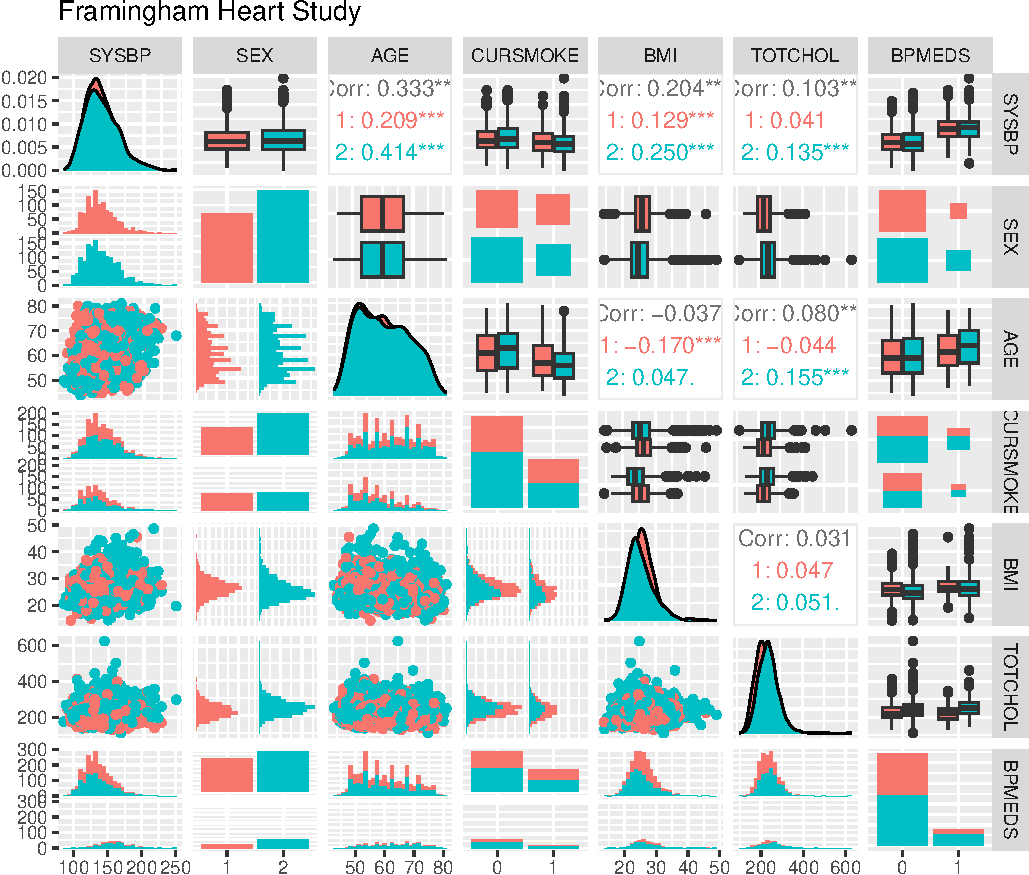
\includegraphics[width=1\linewidth]{1Intro_files/figure-beamer/CVDread-1} \end{center}

What does this plot show?

Red: male; turquoise: female
\end{frame}

\begin{frame}[fragile]
\begin{itemize}
\tightlist
\item
  Diagonal: density plot (generalization of histogram), or barplot.
\item
  Lower diagonals: scatterplot, histograms
\item
  Upper diagonals: correlations, boxplots or barplots
\end{itemize}

\vspace{2mm}

We use \texttt{sex} to color the graph.
\end{frame}

\begin{frame}
\begin{block}{Etiology of CVD}
\protect\hypertarget{etiology-of-cvd}{}
\vspace{3mm}

The question: \textbf{What are the factors that cause high SBP?}

\vspace{2mm}

\(\rightarrow\) we are interested in \emph{inference} (explanation), not
prediction!

\vspace{4mm}

\begin{itemize}
\tightlist
\item
  A \emph{multiple normal linear regression model} was fit to the data
  set with \[-\frac{1}{\sqrt{\texttt{SYSBP}}}\] as response (output) and
  all the other variables as covariates (inputs).
\end{itemize}

\vspace{2mm}

\begin{itemize}
\tightlist
\item
  The results are used to formulate hypotheses about the etiology of CVD
  - to be studied in new trials.
\end{itemize}
\end{block}
\end{frame}

\begin{frame}[fragile]
\scriptsize

\begin{Shaded}
\begin{Highlighting}[]
\NormalTok{modelB}\OtherTok{=}\FunctionTok{lm}\NormalTok{(}\SpecialCharTok{{-}}\DecValTok{1}\SpecialCharTok{/}\FunctionTok{sqrt}\NormalTok{(SYSBP)}\SpecialCharTok{\textasciitilde{}}\NormalTok{SEX}\SpecialCharTok{+}\NormalTok{AGE}\SpecialCharTok{+}\NormalTok{CURSMOKE}\SpecialCharTok{+}\NormalTok{BMI}\SpecialCharTok{+}\NormalTok{TOTCHOL}\SpecialCharTok{+}\NormalTok{BPMEDS,}\AttributeTok{data=}\NormalTok{thisds)}

\FunctionTok{summary}\NormalTok{(modelB)}
\end{Highlighting}
\end{Shaded}

\begin{verbatim}
## 
## Call:
## lm(formula = -1/sqrt(SYSBP) ~ SEX + AGE + CURSMOKE + BMI + TOTCHOL + 
##     BPMEDS, data = thisds)
## 
## Residuals:
##        Min         1Q     Median         3Q        Max 
## -0.0207366 -0.0039157 -0.0000304  0.0038293  0.0189747 
## 
## Coefficients:
##               Estimate Std. Error t value Pr(>|t|)    
## (Intercept) -1.106e-01  1.342e-03 -82.413  < 2e-16 ***
## SEX2        -2.989e-04  2.390e-04  -1.251 0.211176    
## AGE          2.378e-04  1.434e-05  16.586  < 2e-16 ***
## CURSMOKE1   -2.504e-04  2.527e-04  -0.991 0.321723    
## BMI          3.087e-04  2.955e-05  10.447  < 2e-16 ***
## TOTCHOL      9.288e-06  2.602e-06   3.569 0.000365 ***
## BPMEDS1      5.469e-03  3.265e-04  16.748  < 2e-16 ***
## ---
## Signif. codes:  0 '***' 0.001 '**' 0.01 '*' 0.05 '.' 0.1 ' ' 1
## 
## Residual standard error: 0.005819 on 2593 degrees of freedom
## Multiple R-squared:  0.2494, Adjusted R-squared:  0.2476 
## F-statistic: 143.6 on 6 and 2593 DF,  p-value: < 2.2e-16
\end{verbatim}

\normalsize
\end{frame}

\begin{frame}[fragile]{Example 2: Classification (iris plants)}
\protect\hypertarget{example-2-classification-iris-plants}{}
The \texttt{iris} flower data set is a very famous multivariate data set
introduced by the British statistician and biologist Ronald Fisher in
1936.

\(~\)

The data set contains

\begin{itemize}
\tightlist
\item
  \textbf{three plant species} \{setosa, virginica, versicolor\}
\item
  \textbf{four features measured} for each corresponding sample:

  \begin{itemize}
  \tightlist
  \item
    \texttt{Sepal.Length}
  \item
    \texttt{Sepal.Width}
  \item
    \texttt{Petal.Length}
  \item
    \texttt{Petal.Width}.
  \end{itemize}
\end{itemize}
\end{frame}

\begin{frame}
\begin{figure}
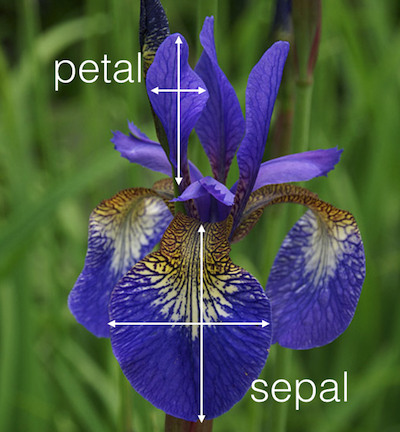
\includegraphics[width=150pt]{iris} \caption{Iris plant with sepal and petal leaves}\label{fig:iris_pic}
\end{figure}

\tiny

\url{http://blog.kaggle.com/2015/04/22/scikit-learn-video-3-machine-learning-first-steps-with-the-iris-dataset/}
\end{frame}

\begin{frame}[fragile]
\scriptsize

\begin{Shaded}
\begin{Highlighting}[]
\FunctionTok{head}\NormalTok{(iris)}
\end{Highlighting}
\end{Shaded}

\begin{verbatim}
##   Sepal.Length Sepal.Width Petal.Length Petal.Width Species
## 1          5.1         3.5          1.4         0.2  setosa
## 2          4.9         3.0          1.4         0.2  setosa
## 3          4.7         3.2          1.3         0.2  setosa
## 4          4.6         3.1          1.5         0.2  setosa
## 5          5.0         3.6          1.4         0.2  setosa
## 6          5.4         3.9          1.7         0.4  setosa
\end{verbatim}

\normalsize
\end{frame}

\begin{frame}
Aim: correctly classify the species of an iris plant from sepal length
and sepal width.

\includegraphics{1Intro_files/figure-beamer/iriscont-1.pdf}
\end{frame}

\begin{frame}
\begin{block}{Linear boundaries}
\protect\hypertarget{linear-boundaries}{}
\vspace{2mm}

In this plot the small black dots represent correctly classified iris
plants, while the red dots represent misclassifications. The big black
dots represent the class means.

~

\includegraphics[width=10cm]{1Intro_files/figure-beamer/irislda-1}
\end{block}
\end{frame}

\begin{frame}
\begin{block}{Non-linear boundaries}
\protect\hypertarget{non-linear-boundaries}{}
\vspace{2mm}

Sometimes a non-linear boundary is more suitable.

\(~\)

\includegraphics[width=10cm]{1Intro_files/figure-beamer/irisqda-1}
\end{block}
\end{frame}

\begin{frame}{Example 3: Unsupervised methods (Gene expression)}
\protect\hypertarget{example-3-unsupervised-methods-gene-expression}{}
(Check also the gene expression example in chapter 1 of the course book)

\vspace{2mm}

\begin{itemize}
\tightlist
\item
  The relationship between inborn maximal oxygen uptake and skeletal
  muscle gene expression was studied.
\end{itemize}

\vspace{1mm}

\begin{itemize}
\tightlist
\item
  Rats were artificially selected for high and low running capacity (HCR
  and LCR, respectively).
\end{itemize}

\vspace{1mm}

\begin{itemize}
\tightlist
\item
  Rats were either kept sedentary or trained.
\end{itemize}

\vspace{1mm}

\begin{itemize}
\tightlist
\item
  Transcripts significantly related to running capacity and training
  were identified.
\end{itemize}

\vspace{1mm}

\begin{itemize}
\tightlist
\item
  Heat maps showing the expression level for the most significant
  transcripts were presented graphically.
\end{itemize}

\vspace{1mm}

\begin{itemize}
\tightlist
\item
  This is \emph{hierarchical cluster analysis} with pearson correlation
  distance measure (module 10).
\end{itemize}
\end{frame}

\begin{frame}
\begin{figure}
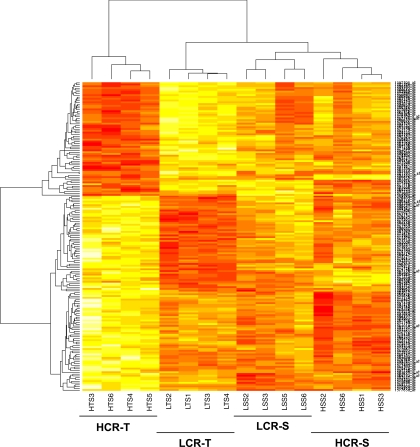
\includegraphics[width=150pt]{heatmap} \caption{Heat map of the most significant transcripts. Transcripts with a high expression are shown in red and transcripts with a low expression are shown in yellow.}\label{fig:heatmap_pic}
\end{figure}

\tiny

More: \url{https://www.ncbi.nlm.nih.gov/pmc/articles/PMC2585023/}
\end{frame}

\begin{frame}{Example 3: Unsupervised learning}
\protect\hypertarget{example-3-unsupervised-learning}{}
\textbf{Q}: What is different in this example?

\pause

\begin{itemize}
\tightlist
\item
  We do not have a response variable
\item
  We are not interested in predicting a particular variable but in
  determining whther there are groups, or clusters, among the
  observations.
\end{itemize}
\end{frame}

\begin{frame}{Examples of unsupervised learning in practice}
\protect\hypertarget{examples-of-unsupervised-learning-in-practice}{}
\begin{itemize}
\item
  Cancer research: Look for subgroups within the patients or within the
  genes in order to better understand the disease
\item
  Online shopping site: Identify groups of shoppers as well as groups of
  items within each of those shoppers groups.
\item
  Search engine: Search only a subset of the documents in order to find
  the best one for retrieval.
\item
  \(\dots\)
\end{itemize}
\end{frame}

\begin{frame}{Plan for rest of the week}
\protect\hypertarget{plan-for-rest-of-the-week}{}
\(~\)

\begin{itemize}
\tightlist
\item
  You can work through parts 1 - 6 in the R course
  \url{https://digit.ntnu.no/courses/course-v1:NTNU+IE-IMF+2023_AUG/about}
\end{itemize}

\vspace{2mm}

\begin{itemize}
\tightlist
\item
  Ideally use your Feide account to log in.
\end{itemize}

\vspace{2mm}

\begin{itemize}
\tightlist
\item
  There is a discussion forum (click on the ``Discussion'' tab).
\end{itemize}
\end{frame}

\begin{frame}{Getting started with R}
\protect\hypertarget{getting-started-with-r}{}
\vspace{2mm}

\begin{itemize}
\tightlist
\item
  Install R (use the Norwegian CRAN mirror):
  \url{https://www.r-project.org}
\end{itemize}

\vspace{2mm}

\begin{itemize}
\tightlist
\item
  Install Rstudio \url{https://www.rstudio.com/products/rstudio/}
\end{itemize}

\vspace{4mm}

If you need help on installing R and RStudio on you laptop computer,
contact \href{mailto:orakel@ntnu.no}{\nolinkurl{orakel@ntnu.no}}.
\end{frame}

\begin{frame}
\begin{block}{Some additional links}
\protect\hypertarget{some-additional-links}{}
\vspace{4mm}

\begin{enumerate}
[1)]
\item
  What is R? \url{https://www.r-project.org/about.html} \vspace{2mm}
\item
  What is RStudio? \url{https://www.rstudio.com/products/rstudio/}
  \vspace{2mm}
\item
  What is CRAN? \url{https://cran.uib.no/} \vspace{2mm}
\end{enumerate}
\end{block}
\end{frame}

\begin{frame}
\begin{block}{Additional nice R resources}
\protect\hypertarget{additional-nice-r-resources}{}
\(~\)

\begin{itemize}
\tightlist
\item
  Grolemund and Hadwick (2017): ``R for Data Science'',
  \url{http://r4ds.had.co.nz}
\end{itemize}

\vspace{2mm}

\begin{itemize}
\tightlist
\item
  Hadwick (2009): ``ggplot2: Elegant graphics for data analysis''
  textbook: \url{https://ggplot2-book.org/}
\end{itemize}

\vspace{2mm}

\begin{itemize}
\tightlist
\item
  \href{https://www.rstudio.com/resources/cheatsheets/}{Overview of
  cheat sheets from RStudio}
\end{itemize}

\vspace{2mm}

\begin{itemize}
\tightlist
\item
  Questions on R: ask the course staff, colleagues, and
  \href{https://stackoverflow.com/}{stackoverflow}.
\end{itemize}
\end{block}
\end{frame}

\end{document}
